\chapter{AccessibleHub: Transforming mobile accessibility guidelines into code}
\label{chap:accessibility-toolkit}

\chapterintroline{
    This chapter presents an accessibility-focused learning toolkit, which is an all-encompassing guide to mobile application developers. It extends Gaggi's research implemented by Budai's work into Flutter accessibility and gives a more focused approach to orient the developers themselves in how to actually implement an accessible mobile application. Here \textit{AccessibleHub} is introduced, an interactive learning toolkit built using \gls{reactnative}, which aims to enhance accessibility implementation through hands-on examples, component-level guidance, and comparative insights between React Native and \gls{flutter}. By providing a structured educational approach grounded in \gls{wcagg} principles and mobile-specific considerations, AccessibleHub empowers developers to bridge the gap between accessibility guidelines and real-world implementation. 
}

\section{Introduction}
\label{sec:intro}

\subsection{Challenges in implementing accessibility guidelines}

The importance of mobile app accessibility extends beyond mere compliance with legal regulations. Ensuring equal access to digital content and services is not only an ethical obligation but also a smart business decision. By prioritizing accessibility, app developers and companies can tap into a larger user base, improve user satisfaction, and demonstrate their commitment to social responsibility.
Despite the clear benefits and moral imperatives of mobile app accessibility, many developers still struggle to effectively implement accessibility guidelines in their projects. The \acrshort{wcagacr}, developed by the \gls{w3cg}, serve as the international standard for digital accessibility. However, translating these guidelines into practical implementation can be a challenging task, particularly starting from pure formal guidelines into everyday code. \\

One of the primary challenges lies in the complexity of the guidelines themselves. WCAG encompasses a wide range of \textit{success criteria}, organized under four main general \textit{principles}: perceivable, operable, understandable, and robust. Each principle contains multiple guidelines, and each guideline has several success criteria at different levels of \textit{conformance} (A, AA, AAA). Navigating this intricate web of requirements and understanding how to apply them to specific mobile app components can be overwhelming for developers, especially those new to accessibility. 
Moreover, the practical implementation of accessibility guidelines often varies across different platforms and frameworks. \textit{iOS} and \textit{Android}, the two dominant mobile operating systems, have their own unique accessibility \textit{API}s, tools, and best practices. Cross-platform frameworks like React Native and Flutter add another layer of complexity, as developers must ensure that their accessibility implementations are compatible with the underlying platform-specific mechanisms. \\ 

Furthermore, there is often a lack of clear, practical examples and guidance on how to implement accessibility features in real-world mobile app projects. While the \textit{WCAG} provides a solid foundation, it is primarily focused on web content and may not always directly address the unique challenges and interaction patterns of mobile apps. Developers often struggle to bridge the gap between the theoretical guidelines and the specific implementation details required for their projects.

\subsection{The need for practical developer education}

To address these challenges and bridge the gap between accessibility guidelines and practical implementation, there is a pressing need for developer education resources that focus on real-world, hands-on learning experiences. Traditional documentation and guidelines, while valuable, often fall short in providing the level of detail and interactivity needed to effectively guide developers through the accessibility implementation process.
This is where the concept of an \textit{accessibility learning toolkit} comes into play. An accessibility toolkit is designed to serve as a comprehensive, interactive resource that empowers developers to create accessible mobile applications by providing:

\begin{enumerate}
    \item Clear explanations of \acrshort{wcagacr} guidelines and their applicability to mobile apps;
    
    \item Step-by-step implementation guidance for common mobile app components and interaction patterns;
    
    \item Practical code examples and tutorials that demonstrate best practices;
    
    \item Hands-on exercises and challenges to reinforce learning and build confidence;
    
    \item Tools and techniques for testing and validating the accessibility of mobile apps.
\end{enumerate}

The primary goal of an accessibility learning toolkit is to bridge the gap between the theoretical knowledge of accessibility guidelines and the practical skills needed to implement them effectively in real-world projects. 
The toolkit should cater to developers at various levels of expertise, from beginners who are new to accessibility concepts to experienced professionals seeking to deepen their knowledge and stay up-to-date with the latest best practices. By providing a comprehensive, hands-on learning resource, the accessibility toolkit can play a crucial role in promoting a culture of inclusive design and development within the mobile app industry. \\

Current research, including Budai's work on Flutter accessibility testing, has primarily focused on end-user validation and testing methodologies. However, developers need practical, implementation-focused guidance that bridges multiple frameworks and platforms.
Despite widespread accessibility guidelines and standard, mobile application developers face significant challenges in translating theoretical requirements into practical implementations. This gap between guidelines and implementation is particularly evident in mobile development, where different platforms, screen sizes, and interaction models add complexity to accessibility implementation. Some of the most common challenges include:

\begin{itemize}
    \item Complex testing requirements - developers must validate across multiple devices, \gls{screenreaderg}, and interaction modes;
    
    \item Framework-specific implementations - each platform has unique accessibility \gls{apig}s and requirements;
    
    \item Limited practical examples - most documentation focuses on theoretical guidelines rather than concrete implementation patterns;
    
    \item Performance considerations - accessibility features must be implemented without compromising app performance.
\end{itemize}

Effective developer education in accessibility requires a solid grounding in learning theories that emphasize hands-on, interactive approaches. By integrating established learning theories with technical education principles, it's possible to justify the interactive and practical approach adopted in this toolkit. In doing so, we draw on constructivist and experiential learning models, which have been widely recognized as effective frameworks in technical and developer education.

Constructivist learning theories, pioneered by Piaget \cite{piaget1970science} and Vygotsky \cite{vygotsky1978mind}, posit that learning is an active process in which individuals construct knowledge based on their prior experiences and interactions with the environment. In the context of developer education, this suggests that hands-on learning is more effective than passive instruction \cite{savery2006overview}. By engaging with real-world accessibility challenges and actively experimenting with code implementations, developers can build a deeper understanding of accessibility guidelines and best practices, by having a tool at their disposal easy to use and to navigate. \\

Kolb's \textit{Experiential Learning Theory} \cite{kolb1984experiential} further supports this approach by describing learning as a four-stage cycle: concrete experience, reflective observation, abstract conceptualization, and active experimentation. For developers learning about accessibility, this cycle might involve encountering accessibility issues in their projects, analyzing existing solutions and guidelines, synthesizing their understanding of \acrshort{wcagacr} principles, and applying these principles to their own code. \textit{AccessibleHub} facilitates this learning cycle by providing a structured, interactive environment for developers to engage with accessibility concepts and implementations being organized into different core sections. By aligning with these proven pedagogical approaches, \textit{AccessibleHub} aims to provide an effective and engaging learning experience for developers. Moreover, by fostering a community of practice around accessibility while providing easier access to learning resources, this project encourages ongoing learning and knowledge sharing among developers, promoting the continuous improvement and dissemination of accessibility best practices.

\subsection{Research objectives and methodology}

Building upon previous research into mobile accessibility, this work aims to provide a comprehensive understanding of accessibility implementation across major cross-platform frameworks. While existing research indeed set grounds for both guidelines on accessibility and testing methodologies, there is a critical need to understand how these guidelines translate into practice for developers. 

This research addresses three fundamental questions about accessibility implementation in mobile development frameworks (referring to these ones as \textit{research questions}, following the work in \cite{perinello2024accessibility}:

\begin{itemize}
    \item First, we investigate whether components and widgets provided by frameworks are \textit{accessible by default}, without requiring additional developer intervention. This analysis is crucial for understanding the baseline accessibility support provided by each framework and identifying areas where additional implementation effort may be required;
    
    \item Second, we examine the \textit{feasibility of making non-accessible components accessible} through additional development effort. This involves analyzing the technical capabilities of each framework and identifying the necessary modifications to achieve accessibility compliance;
    
    \item Third, we quantify the \textit{development overhead required to implement accessibility features} when they are not provided by default. This includes measuring additional code requirements, analyzing complexity increases, and evaluating the impact on development workflows.
\end{itemize}

These questions is addressed via the usage of a systematic methodology aiming to address in detail accessibility support in React Native and Flutter, focusing on component implementation patterns and native platform integration. The implementation is comparative, allowing developers to directly implement accessible code examples with different degrees of implementation complexity measured quantitatively (including lines of code, required properties, and additional components needed for accessibility support). Comprehensive testing of implementations is also done using screen readers and other assistive technologies to verify accessibility compliance.

The \textit{goal} is to create an accessible application that serves three key purposes:
\begin{enumerate}
    \item To provide developers with practical, interactive examples of accessibility implementation, able to be copied easily and ported inside of other projects;
    
    \item To compare and contrast accessibility approaches between the main cross-development mobile frameworks in the current mobile landscape;
    
    \item To establish a reusable pattern library that demonstrates engine architecture, widget systems, and native platform integration, while ensuring compliance with current accessibility guidelines and legal requirements.
\end{enumerate}

The following sections will detail the development of \textit{AccessibleHub}, an application developed in React Native designed to serve as a practical manual for implementing accessibility features. While the technical aspects of cross-platform frameworks will be discussed later, the focus remains on providing developers with actionable implementation patterns and comparative insights for building accessible applications.

\section{React Native Overview}
\label{sec:reactnative-overview}

\gls{reactnative} is an open-source framework developed by Meta that enables developers to build mobile applications using JavaScript and the React paradigm (\cite{site:reactnative}). It employs a declarative, component-based approach through the use of \textit{JSX}, which is an XML-like syntax that allows developers to intermix JavaScript logic with markup. This combination not only improves code readability but also enhances modularity and facilitates code reuse.

\begin{figure}[ht]
    \centering
    
\includegraphics[width=0.4\textwidth, alt={React Native Logo}]{img/react-native-logo.png}
    \caption{React Native Logo}
    \label{fig:reactnative-logo}
\end{figure}

\subsection{Core architecture and features}
\begin{itemize}
    \item \textit{Component-based architecture:}  
    The entire user interface in React Native is built from reusable components. Each component encapsulates its own logic and presentation, which greatly aids in the maintainability and scalability of complex applications;
    
    \item \textit{JSX syntax:}  
    Developers write the \acrshort{ui} using \textit{JSX}, a syntax extension similar to \textit{HTML}. This blending of code and layout simplifies the development process and enables a more intuitive understanding of the component structure;
    
    \item \textit{Bridging mechanism:}  
    React Native’s bridge enables asynchronous communication between the JavaScript layer and native modules. This means that while the application is written in JavaScript, performance-critical tasks can be executed using native code (e.g., Objective-C, Swift, or Java), ensuring a native look and feel without sacrificing performance;
    
    \item \textit{Hot reloading:}  
    One of the standout features present in this framework, which allows developers to see changes in real time without restarting the entire application. This accelerates the development cycle and aids in rapid prototyping;
    
    \item \textit{Unified codebase:}  
    React Native enables the development of applications for both iOS and Android using a single codebase. This unified approach reduces development time and effort compared to maintaining separate codebases for each platform.
\end{itemize}

\subsection{Accessibility in React Native}
React Native provides a robust set of accessibility features that are deeply integrated into its component model. This allows developers to create inclusive applications without relying on external libraries or writing platform-specific code (following what's present into \cite{site:reactnativeaccess}). Here are the key accessibility features in React Native:

\begin{itemize}
    \item \textbf{Accessibility properties}: React Native components can be enhanced with a variety of accessibility properties that provide semantic meaning and context for assistive technologies. These properties include:
    \begin{itemize}
        \item \texttt{accessibilityLabel}: A concise, descriptive string that identifies the component for screen reader users;
        \item \texttt{accessibilityRole}: Defines the component's semantic role (e.g., \texttt{"button"}, \texttt{"header"}), helping assistive technologies interpret its purpose correctly;
        \item \texttt{accessibilityHint}: Provides additional context about a component's function or the result of interacting with it;
        \item \texttt{accessibilityState}: Describes the current state of a component (e.g., \texttt{selected}, \texttt{disabled}), which is essential for conveying dynamic changes.
    \end{itemize}
    
    \item \textbf{Accessibility actions}: React Native allows developers to define custom accessibility actions for components, enabling advanced interactions beyond the default gestures. For example, a custom \texttt{accessibilityAction} could be added to a component to trigger a specific behavior when activated by an assistive technology;
    
    \item \textbf{Accessibility focus}: React Native manages accessibility focus automatically, ensuring that the correct component receives focus when navigating with assistive technologies. Developers can also programmatically control focus using the \texttt{accessibilityElementsHidden} and \\\texttt{importantForAccessibility} properties;
    
    \item \textbf{Accessibility events}: React Native provides accessibility events that notify assistive technologies when important changes occur in the application. These events include:
    \begin{itemize}
        \item \texttt{onAccessibilityTap}: Called when a user double-taps a component while using an assistive technology;
        \item \texttt{onMagicTap}: Called when a user performs the "magic tap" gesture (a double-tap with two fingers) to activate a component;
        \item \texttt{onAccessibilityFocus}: Called when a component receives accessibility focus;
        \item \texttt{onAccessibilityBlur}: Called when a component loses accessibility focus.
    \end{itemize}
\end{itemize}

By leveraging these built-in accessibility features, developers can create React Native applications that are inclusive and accessible to users with diverse needs and abilities. The tight integration of accessibility into the core component model ensures that developers can create accessible apps without sacrificing performance or maintainability.

\subsection{Advantages and developer benefits}

Using React Native offers several benefits for developers, briefly listed here:
\begin{itemize}
    \item \textit{Rapid development:}  
    Thanks to hot reloading and a vast ecosystem of reusable components, developers can iterate quickly and efficiently;
    
    \item \textit{Cross-platform consistency:}  
    With a unified codebase for both iOS and Android, developers can ensure a consistent user experience without duplicating effort;
    
    \item \textit{Integrated accessibility:}  
    React Native’s direct integration of accessibility properties allows developers to implement accessible features without having to rely on external tools or write platform-specific code;
    
    \item \textit{Community and support:}  
    A large and active community means extensive documentation, a wealth of third-party libraries, and a robust support network for troubleshooting and enhancements;
    
    \item \textit{Seamless transition for web developers:}  
    Developers familiar with React for web applications will find the transition to React Native smooth, as the core concepts and \textit{JSX} syntax remain consistent.
\end{itemize}

\subsection{Differences from native iOS/Android and web development}
\begin{itemize}
    \item \textit{Native iOS/Android:}  
    In native development, accessibility is handled through platform-specific \gls{apig}: \gls{voiceover} on \textit{iOS} and \gls{talkback} on \textit{Android}, which require different tools and approaches. React Native provides a unified \textit{API}s, streamlining the implementation of accessibility features across both platforms.
    
    \item \textit{Web development:}  
    Whereas web accessibility is achieved by adding \gls{ariag} attributes to \textit{HTML}, React Native integrates accessibility directly within its component structure. This intrinsic approach treats accessibility as a core attribute of each component, rather than an external addition.
\end{itemize}

In summary, React Native offers a modern, efficient, and developer-friendly environment that not only simplifies cross-platform mobile development but also incorporates accessibility into its core design. This makes it an ideal choice for creating inclusive applications, and it forms the foundational platform upon which the \textit{AccessibleHub} toolkit is built.

\section{AccessibleHub: An Interactive Learning Toolkit}
\label{sec:accessiblehub}

\subsection{Core architecture and design principles}

\textit{AccessibleHub} is a React Native application designed to serve as an interactive manual for implementing accessibility features in mobile development. Unlike traditional documentation or testing frameworks, the application provides developers with hands-on examples and implementation patterns that can be directly applied to their projects.

The application is structured around four conceptual main sections:
\begin{enumerate}
    \item \textit{Component examples}: Interactive demonstrations of common \acrshort{ui} elements with proper accessibility implementations, including buttons, forms, media content, and navigation patterns. This allows developers to clearly see the implementation of an accessible component and easily copy the code to their convenience;
    
    \item \textit{Framework comparison}: A detailed analysis of accessibility implementation approaches between React Native and Flutter, highlighting differences in component structure, properties, and required code;
    
    \item \textit{Testing tools}: Built-in utilities for validating accessibility features, allowing developers to understand how screen readers and other assistive technologies interact with their implementations;
    
    \item \textit{Implementation guidelines}: Technical documentation that connects WCAG requirements to practical code examples, providing clear paths for meeting accessibility standards.
\end{enumerate}

Each component presented serves dual purposes: demonstrating proper accessibility implementation while providing reusable code patterns. The application emphasizes practical implementation over theoretical guidelines, showing developers not just what to implement effectively. By focusing on developer experience, \textit{AccessibleHub} bridges the gap between accessibility requirements and actual implementation, providing a resource that can be directly integrated into the development workflow. \\

The \textit{design} philosophy of \textit{AccessibleHub} is founded on principles that bridge theoretical accessibility guidelines with practical implementation needs. While analyzing the current landscape of mobile development frameworks and accessibility implementation presented in \ref{chap:accessibility-literature}, a clear pattern emerges: developers need more practical, implementation-focused guidance that directly addresses the complexity of building accessible applications. To address this need, \textit{AccessibleHub} adopts three fundamental architectural principles:

\begin{enumerate}
    \item The usage of a \textit{component-first architecture}, where each UI element exists as an independent, self-contained unit demonstrating both implementation patterns and accessibility features. In other words, each one of them is being constructed within an \textit{accessibility-first} experience which ensures that usage of screen readers and other assistive technologies is kept as a priority. This modular approach provides two advantages: it first allows developers to comprehend and apply accessibility features in isolation, hence reducing cognitive load and implementation complexity, and enables systematic testing and validation of accessibility features of every component. Also, this means accessibility patterns can be studied, implemented, and verified in isolation from added complexity brought in by interactions among those components;

    \item \textit{Progressive enhancement} as a core design methodology. Instead of presenting accessibility as big challenge from the start, components are structured in increasing levels of complexity. This starts with basic elements like buttons and text inputs where basic accessibility patterns can be established. As developers master these foundational components, the application introduces more complex patterns such as forms, navigation systems, and gesture-based interactions. This helps into guiding the development towards more complicated scenarios;

    \item Focus on \textit{framework-agnostic patterns}, not depending on a specific framework while providing concrete code implementations. Even though \textit{AccessibleHub} has been implemented in React Native, all the patterns and principles explained are designed to transcend into specific framework implementations. The approach wants to give importance to the compatibility and reusability in the framework on the mobile development side. It will compare the implementations, mainly between React Native and Flutter, to show how developers can port accessibility patterns across different frameworks and understand core accessibility concepts in an easy-to-implement manner within professional projects. 
    
\end{enumerate}

Through these principles, \textit{AccessibleHub} aims to transform accessibility from an afterthought into an \textit{accessibility-by-design}. The application serves not just as a reference implementation, but as an educational tool that guides developers through the process of building truly accessible applications. This approach recognizes that effective accessibility implementation requires both theoretical understanding and practical experience, providing developers with the tools they need to create more inclusive mobile applications.

\subsection{Educational framework design}

\textit{AccessibleHub}'s educational framework is designed to provide a structured, incremental learning experience that progressively builds accessibility knowledge and skills. The content is organized into different \textit{learning modules}, each focusing on a key aspect of mobile accessibility. This is structured incrementally, so to help a developer gather a general idea on what needs to be implemented following a practical roadmap of steps: this allows to focus on different aspects of mobile accessibility, selecting each time the most relevant ones.

The core of the application is divided into different main screens, following:

\begin{enumerate}
    \item \textbf{Home} - The entry point for the \textit{AccessibleHub} application. It provides an overview of the main sections and guides users on where to start their accessibility learning journey. The Home screen is designed to be intuitive and user-friendly, with clear call-to-action towards the accessible components section, allowing a developer or a user navigate to the desired section from the Home screen, comprehensive of comparison between the main mobile frameworks, learn about best practices in mobile accessibility and access testing tools documentation. There is also present a compliance dashboard provides an overview of an app's accessibility compliance status, based on the \acrshort{wcagacr} and \acrshort{mcagacr} guidelines. Developers can use this information to prioritize their accessibility efforts and focus on the areas that need the most attention;

    \item \textbf{Accessible Components} - Developers can learn how to implement accessible UI components in their mobile applications. This section is divided into four subscreens, each focusing on a specific category of components:

    \begin{itemize}
        \item \textit{Buttons and Touchables}: It covers the implementation of accessible buttons and touchable elements. It provides code examples and best practices for ensuring that these interactive elements are perceivable, operable, and understandable by all users, including those with disabilities;

        \item \textit{Forms}: The subscreen focuses on creating accessible input forms, including text fields, checkboxes, radio buttons, and date/time pickers. It demonstrates how to properly label form elements, provide instructions and feedback, and ensure that forms can be navigated and completed using various input methods, such as keyboards and screen readers;

        \item \textit{Media}: In the Media subscreen, developers learn how to make media content, such as images, videos, and audio, accessible to users with visual or auditory impairments. This includes providing alternative text for images, captions for videos, and transcripts for audio content;

        \item \textit{Dialogs}: It covers the creation of accessible modal dialogs, popups, and alerts. It provides guidance on how to ensure that these elements are properly announced by screen readers, can be easily dismissed, and do not interfere with the user's ability to navigate the application, maintaining focus management and ensuring clear exit strategies;

       \item \textit{Advanced}: This particular subscreen covers elements like alerts, sliders, progress bars and tab navigation, analyzing how accessibility may regard different animated or interactive components for more complex gesture interactions used everyday by users.
    \end{itemize}

Throughout the Components section, code implementations are shared as examples, which developers can easily copy to their clipboard and integrate into their own projects. This hands-on approach allows developers to quickly apply the accessibility principles they learn and see the results in action.

\item \textbf{Best Practices} - Designed to give developers a general understanding of the overarching principles and guidelines for creating accessible mobile applications. It is divided into five subscreens, each addressing a key aspect of mobile accessibility:

    \begin{itemize}
        \item \textit{Gestures Tutorial}: This subscreen provides an overview of the various gesture interactions used in mobile applications and how to make them accessible to users with motor impairments or those relying on assistive technologies. It covers best practices for implementing alternative input methods and providing clear instructions and feedback. These gestures are general, tested to be used universally, both by everyday users and screen reader ones;

        \item \textit{Semantics Structure}: Here, developers learn about the importance of using semantic \textit{HTML} and \gls{ariag} roles to convey the structure and meaning of the application's content. This helps screen readers and other assistive technologies better understand and navigate the application;

        \item \textit{Navigation}: This one focuses on creating accessible navigation patterns, such as menus, tabs, and breadcrumbs. It provides guidance on how to ensure that navigation elements are properly labeled, can be operated using various input methods, and provide clear feedback to the user, jumping directly to the main context of a screen and bringing the attention to an element on-screen without distracting him from the action to be completed;

        \item \textit{Screen Reader Support}: This subscreen covers the specific considerations for making mobile applications compatible with screen readers, such as \gls{voiceover} on \textit{iOS} and \gls{talkback} on \textit{Android}. It includes best practices for labeling elements, providing alternative text, and ensuring that the application's content and functionality can be fully accessed and understood using a screen reader;

        \item \textit{Accessibility Guidelines}: The Accessibility Guidelines subscreen provides an overview of the key accessibility standards to be followed and a general list of principles to incorporate into a project, seeing how they apply to mobile application development. It helps developers understand the different levels of conformance and how to assess their application's accessibility against these guidelines.
    \end{itemize}

\item \textbf{Framework Comparison} - It provides a side-by-side comparison of the accessibility features and implementation differences between popular mobile development frameworks, such as React Native and Flutter. This section helps developers understand how accessibility is handled in each framework and provides guidance on leveraging the specific accessibility APIs and tools available in each one. By highlighting the similarities and differences between frameworks, developers can make informed decisions about which framework to use for their accessibility needs and how to optimize their implementations for each platform;

\item \textbf{Tools} - It serves as a central hub for accessing various accessibility-related tools and resources. This includes links to official documentation, such as the React Native Accessibility \acrshort{api} reference and the \textit{Flutter Accessibility package} documentation. It also provides quick access to popular accessibility testing tools, such as \textit{Accessibility Scanner} for \textit{Android} and \textit{Accessibility Inspector} for \textit{iOS}. By consolidating these resources in one place, the Tools screen makes it easy for developers to find the information and tools they need to ensure their applications are fully accessible; 

\item \textbf{Settings} - Allows users to customize various aspects of the \textit{AccessibleHub} application to suit their individual learning needs and preferences. This includes options for adjusting the font size, color contrast (including options for gray scale and dark mode), reduced motion settings and others to help users and ensure the application itself is accessible to a wide range of users. It also provides information on how to configure the accessibility settings on the user's device, such as enabling screen readers or adjusting the display settings. By offering these customization options and guidance, the page reinforces the importance of accessibility as an everyday tool, meant to accompany practical user needs in an easy and quick way;

\item \textbf{Instruction and Community} - It provides a collaborative learning environment that extends beyond technical implementation. This section offers developers an opportunity to dive deeper into accessibility knowledge through curated resources and community engagement allowing for easier exploration towards other online resources. By providing a platform for continuous learning and collaboration, this screen reinforces the importance of accessibility as a collective effort and a fundamental aspect of modern mobile application development.
    
\end{enumerate}

\subsection{From guidelines to implementation: a screen-based methodology}

Accessibility guidelines and standards - most notably the \acrshort{wcagacr}  and related mobile-specific considerations—establish the formal foundation for inclusive digital design. These criteria are essential but inherently abstract and can be challenging to implement directly in code. Building on Perinello and Gaggi's approach focusing solely on post-implementation testing, the methodology presented embeds accessibility into the development process. We do this by analyzing each screen of the application through a structured framework that connects theoretical requirements with practical implementation strategies. The approach to be considered is built following these layers:

\begin{enumerate}
    \item \textit{Theoretical foundation} – This layer encompasses the abstract principles and success criteria defined by \textit{WCAG}/\acrshort{mcagacr}. For example, \textit{WCAG}’s four core principles require that content be presented in ways users can perceive, interact with, and understand. These criteria serve as the benchmark for our analysis;

    \item \textit{Implementation pattern} – Here, we translate the abstract requirements into concrete code structures within a mobile development context. In \textit{AccessibleHub}, this involves the systematic use of React Native properties (such as \textit{accessibilityLabel}, \textit{accessibilityRole}, etc.) to ensure that \acrshort{ui} components satisfy the established guidelines;

    \item \textit{User interaction flow} – Finally, we consider how end users interact with these components. This includes the behavior of assistive technologies (like screen readers), proper focus management, and the overall usability of the component within its real-world context.
\end{enumerate}

To illustrate this methodology in practice, we first map the \textit{UI} elements of a representative screen to their corresponding semantic roles. Next, we link each component to the relevant \acrshort{wcagacr} and \acrshort{mcagacr} criteria presented in the previous subsections, noting both the minimum compliance requirements and potential enhancements. Finally, we describe the technical solution—specifically, how React Native accessibility code properties are applied to meet and exceed these standards. This structured approach not only bridges the gap between abstract guidelines and real-world coding tasks but also sets the stage for the more detailed, screen-by-screen analyses presented in the next section.

\section{Accessibility Implementation Guidelines}
\label{sec:implementation-guidelines}

Having established the overall architecture of \textit{AccessibleHub} and the guiding principles from both \textit{WCAG} and \textit{MCAG}, we now present a screen-by-screen analysis. Each subsection highlights the key \textit{success criteria} addressed, references relevant \textit{mobile-specific considerations}, and demonstrates practical solutions in React Native. Where applicable, we contrast these with Flutter's approach, building upon the insights from Budai \cite{budai2024mobile} in Flutter - following guidelines and then giving advice into introducing new ones.

\subsection{Home Screen}

The Home Screen serves as the primary entry point of the \textit{AccessibleHub} application. It provides key metrics on accessibility compliance (e.g., number of accessible components, \acrshort{wcagacr} conformance level) and direct navigation to core sections: \textit{Accessible Components} (Quick Start), \textit{Best Practices}, \textit{Testing Tools}, and the \textit{Framework Comparison}. An example of the interface is shown in Figure ~\ref{fig:home_screens_sidebyside}.

\begin{figure}[ht]
    \centering
    \begin{subfigure}[b]{0.48\textwidth}
        \centering
        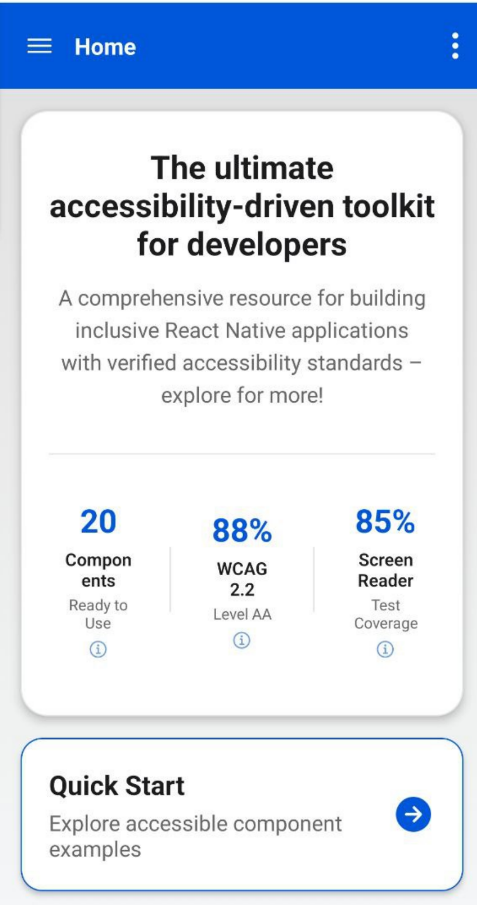
\includegraphics[width=\linewidth, alt={First part of the Home Screen}]{img/home1.png}
        \caption{Home Screen - Part 1}
        \label{fig:home-left}
    \end{subfigure}
    \hfill
    \begin{subfigure}[b]{0.49\textwidth}
        \centering
        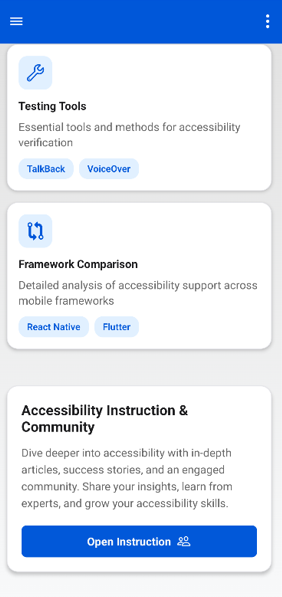
\includegraphics[width=\linewidth, alt={Second part of the Home Screen}]{img/home2.png}
        \caption{Home Screen - Part 2}
        \label{fig:home-right}
    \end{subfigure}
    \caption{Side-by-side view of the two Home sections, with metrics and navigation buttons}
    \label{fig:home_screens_sidebyside}
\end{figure}

Below is a structured analysis referencing both \textit{WCAG 2.2} and mobile-specific guidelines (\textit{MCAG}). Following the approach given by Budai \cite{budai2024mobile}, apart from existing guidelines, new or extended considerations for developers paralleling the approach used, will be given from now on.

\subsubsection{Relevant guidelines and success criteria}

\paragraph{WCAG 2.2}
\begin{itemize}
    \item \textbf{1.4.3 Contrast (Minimum) (Level AA)}\\ 
    The hero title, the displayed metrics (e.g., ``18 Components,'' ``76\% WCAG 2.2''), and the quick start button are designed to meet a minimum contrast ratio of 4.5:1. This ensures that text is easily legible against its background, as verified through both manual and automated methods (e.g., using the \textit{react-native-a11y} plugin).
    
    \item \textbf{2.4.7 Focus Visible (Level AA)}\\ 
    Interactive elements, such as the \texttt{TouchableOpacity} used for the Quick Start button, include a clear focus indicator. This is critical for users who navigate via keyboard or switch devices.
    
    \item \textbf{2.5.8 Target Size (Minimum) (Level AA)}\\ 
    To support users with reduced dexterity, touch targets (buttons and cards) are designed to be at least \textit{24\,px by 24\,px.}
\end{itemize}

\paragraph{MCAG}
\begin{itemize}
    \item \textbf{Touch Interaction and Gestures}\\ 
    The Home Screen employs large, tappable cards for navigation (e.g., Quick Start, Best Practices), thereby facilitating single-finger interaction, a key requirement for mobile accessibility.
    
    \item \textbf{Contextual Usage Scenarios}\\ 
    The implementation supports both light and dark themes, ensuring that the interface adapts to varying ambient lighting conditions—a mobile-specific consideration.
\end{itemize}

\subsubsection{Implementation details in React Native}

The refined code snippet presented in \ref{lst:home-screen-rn} illustrates how the above success criteria are applied in the Home Screen. In addition, several key accessibility metrics are computed to provide real-time feedback on compliance:

\begin{lstlisting}[
  style=ReactNativeStyle,
  caption={Concise Home Screen snippet in React Native}, 
  label={lst:home-screen-rn}, 
  basicstyle=\ttfamily\footnotesize,
  numbers=left,
]
export default function HomeScreen() {
  const router = useRouter();
  const { colors } = useTheme();

  // Example metrics for illustration
  const accessibilityMetrics = {
    componentScore: 89, // e.g., 16/18 components
    wcagCompliance: 76, // e.g., 38/50 success criteria
    testingScore: 85    // average screen reader coverage
  };

  return (
    <ScrollView
      accessibilityRole="scrollview"
      accessibilityLabel="AccessibleHub Home Screen"
    >
      {/* Hero: stats & headings */}
      <View style={styles.heroCard}>
        <Text style={[styles.heroTitle, { color: colors.text }]} accessibilityRole="header">
          Accessibility Toolkit
        </Text>
        <Text style={[styles.heroSubtitle, { color: colors.textSecondary }]}>
          Build inclusive apps with verified standards.
        </Text>
        <View style={styles.statsContainer}>
          {/* Example stat #1 */}
          <View
            style={styles.statCard}
            accessible
            accessibilityRole="text"
            accessibilityLabel={`${accessibilityMetrics.
            componentScore}% accessible components`}
          >
            <Text style={styles.statNumber}>
              {accessibilityMetrics.componentScore}%
            </Text>
            <Text style={styles.statLabel}>Components</Text>
          </View>
          {/* ... other stats ... */}
        </View>
      </View>

      {/* Quick Start Button */}
      <TouchableOpacity
        style={[styles.quickStartCard, { minHeight: 48, minWidth: 150 }]}
        onPress={() => router.push('/components')}
        accessibilityRole="button"
        accessibilityLabel="Quick Start: accessible component examples"
        accessibilityHint="Navigate to components"
      >
        <Text style={styles.quickStartTitle}>Quick Start</Text>
      </TouchableOpacity>
    </ScrollView>
  );
}

\end{lstlisting}

\paragraph{Key observations}
\begin{itemize}
    \item \textbf{Contrast (WCAG 1.4.3):} The text colors (\texttt{colors.text} and \\\texttt{colors.textSecondary}) are chosen to ensure a contrast ratio of at least 4.5:1 against the white background.
    \item \textbf{Focus Visibility (WCAG 2.4.7):} The use of appropriate accessibility roles (e.g., \texttt{header} for the title, \texttt{button} for the Quick Start card) ensures that users navigating via assistive technologies receive clear visual and auditory focus indicators.
    \item \textbf{Touch Target (WCAG 2.5.8):} By specifying minimum dimensions for the Quick Start button (48\,px by 180\,px), we ensure that touch targets are sufficiently large for users with reduced dexterity.
    \item \textbf{Metric Computation:} The computed metrics provide a quick quantitative overview of accessibility:
    \begin{itemize}
        \item The \textit{Component Score} represents the ratio of accessible components.
        \item The \textit{WCAG Compliance} metric reflects the percentage of success criteria met.
        \item The \textit{Testing Score} aggregates results from screen reader tests.
    \end{itemize}
\end{itemize}

\paragraph{Future enhancements}
The Home Screen is the first point of contact, and as such, it must effectively embody the four pillars of accessibility: Perceivable, Operable, Understandable, and Robust. By integrating computed metrics, the interface not only complies with established guidelines but also provides immediate feedback to developers, encouraging iterative improvements. This approach mirrors Budai’s methodology \cite{budai2024mobile} and offers a practical roadmap for applying \textit{WCAG 2.2} and \textit{MCAG} success criteria in a cross-platform development environment.

Future work may include:
\begin{itemize}
    \item Implementing real-time accessibility monitoring to update metrics dynamically.
    \item Extending this detailed analysis to additional screens and components, with a comparative analysis of additional code required (LOC) for full accessibility compliance.
\end{itemize}

\subsection{Accessible Components Section}

\subsubsection{Relevant guidelines and success criteria}

\paragraph{WCAG 2.2}

\paragraph{MCAG}

\subsubsection{Implementation details in React Native}

\paragraph{Key observations}

\paragraph{Future enhancements}

\subsection{Accessible Component 1}

\subsubsection{Relevant guidelines and success criteria}

\paragraph{WCAG 2.2}

\paragraph{MCAG}

\subsubsection{Implementation details in React Native}

\paragraph{Key observations}

\paragraph{Future enhancements}

\subsection{Best Practices Section}

\subsubsection{Relevant guidelines and success criteria}

\paragraph{WCAG 2.2}

\paragraph{MCAG}

\subsubsection{Implementation details in React Native}

\paragraph{Key observations}

\paragraph{Future enhancements}

\subsection{Best Practice 1}

\subsubsection{Relevant guidelines and success criteria}

\paragraph{WCAG 2.2}

\paragraph{MCAG}

\subsubsection{Implementation details in React Native}

\paragraph{Key observations}

\paragraph{Future enhancements}

\subsection{Framework Comparison}

\subsubsection{Relevant guidelines and success criteria}

\paragraph{WCAG 2.2}

\paragraph{MCAG}

\subsubsection{Implementation details in React Native}

\paragraph{Key observations}

\paragraph{Tools}

\subsection{Best Practice 1}

\subsubsection{Relevant guidelines and success criteria}

\paragraph{WCAG 2.2}

\paragraph{MCAG}

\subsubsection{Implementation details in React Native}

\paragraph{Key observations}

\paragraph{Future enhancements}

\subsection{Settings}

\subsubsection{Relevant guidelines and success criteria}

\paragraph{WCAG 2.2}

\paragraph{MCAG}

\subsubsection{Implementation details in React Native}

\paragraph{Key observations}

\paragraph{Future enhancements}

\subsection{Instruction and Community}

\subsubsection{Relevant guidelines and success criteria}

\paragraph{WCAG 2.2}

\paragraph{MCAG}

\subsubsection{Implementation details in React Native}

\paragraph{Key observations}

\paragraph{Future enhancements}


\newpage

